\documentclass[12pt,a4paper]{article}
\usepackage[ngerman]{babel}
\usepackage[utf8]{vietnam}
\usepackage{amsmath}
\usepackage{amsfonts}
\usepackage{listings}
\usepackage{lmodern}
\usepackage{amssymb}
\usepackage{graphicx}
\usepackage{xifthen}
\usepackage{float}
\usepackage{lastpage}
\usepackage{color}
\usepackage[table,xcdraw]{xcolor}
\usepackage{tabularx}
\usepackage{booktabs}

\usepackage[left=2cm,right=2cm,top=2cm,bottom=2cm]{geometry}
\usepackage{scrextend}
\usepackage{fancyhdr}
\pagestyle{fancy}
\lhead{Lập trình socket}
\rhead{PROXY SERVER}
\setcounter{tocdepth}{1}
%\renewcommand{\thefigure}{\arabic{section}.\arabic{figure}}

\newcommand{\oneline}[1]{%
  \newdimen{\namewidth}%
  \setlength{\namewidth}{\widthof{#1}}%
  \ifthenelse{\lengthtest{\namewidth < \textwidth}}%
  {#1}% do nothing if shorter than text width
  {\resizebox{\textwidth}{!}{#1}}% scale down
}

\renewcommand\tabularxcolumn[1]{>{\centering\arraybackslash}m{#1}}
\newcolumntype{Z}[0]{>{\hsize=1.55\hsize}X}%
\newcolumntype{s}[0]{>{\hsize=.6\hsize}X}%
\newcolumntype{n}[0]{>{\centering\arraybackslash\hsize=1.25\hsize}X}

\begin{document}
	\begin{titlepage}
		\begin{center}
	  		\oneline{\LARGE{TRƯỜNG ĐẠI HỌC KHOA HỌC TỰ NHIÊN - ĐHQG HCM}}
	  		\vskip.1in
	  		
	  		\begin{LARGE}
	  			KHOA CÔNG NGHỆ THÔNG TIN
	  			\vskip.7in
	  			
\includegraphics[scale=.2]{images/logo}
	  			\vskip.7in
	  			MÔN MẠNG MÁY TÍNH
	  			\vskip.2in
	  		\end{LARGE}
	  		
	  		\fontsize{32pt}{44pt}\selectfont BÁO CÁO ĐỒ ÁN\\LẬP TRÌNH SOCKET  		
	  		\vskip2in
	  		
	  		\fontsize{18.5pt}{22pt}\selectfont
	  			Phạm Hải Dương - 19120490
	  			\vskip.05in
	  			Trần Quốc Huy - 19120537
	  			\vskip.05in
	  			Nguyễn Bá Ngọc - 19120603
	  			\vskip0.7in
	  			TP.HCM, ngày \the\day{ }tháng \the\month{ }năm \the\year
		\end{center}
	\end{titlepage}
	\tableofcontents
	\newpage
	\section{Phân công công việc}
		\begin{table}[h]
			%\setlength\aboverulesep{0pt} \setlength\belowrulesep{0pt}
%\setlength\extrarowheight{2pt}
			\begin{tabularx}{\textwidth}{|c|c|X|}
			\hline
			\rowcolor[HTML]{FFDAAE}
			Họ và tên & MSSV & \multicolumn{1}{c|}{\cellcolor[HTML]{FFDAAE}Công việc}                                                                                                                                                                  \\ \hline
			Phạm Hải Dương & 19120490 &
				\begin{itemize}
					\item Cài đặt trích xuất thông tin của web server từ request.
					\item Tìm hiểu ứng dụng của proxy server trong thực tế.
					\item Lập báo cáo.
				\end{itemize}
				\\ \hline
			Trần Quốc Huy & 19120537 & 
				\begin{itemize}
					\item Cài đặt gửi request từ client đến proxy server và từ proxy server đến web server.
					\item Cài đặt việc cấm một host.
					\item Tìm hiểu tài liệu và thiết kế kịch bản cách chạy chương trình.
				\end{itemize}
				 \\ \hline
			Nguyễn Bá Ngọc & 19120603 &
				\begin{itemize}
					\item Cài đặt kiểm tra host có bị cấm hay không.
					\item Cài đặt nhận response từ web server và cuối cùng trả về client.
					\item Xử lý đa luồng.
				\end{itemize}
				\\ \hline
			\end{tabularx}
	\end{table}
	\section{Các biến toàn cục và các hàm chức năng chính}
		\subsection{Các biến toàn cục}
			\begin{itemize}
				\item $HOST$ là địa chỉ IP loopback, do proxy server được cài đặt chung thiết bị với client (127.0.0.1).
				\item $PORT$ là cổng mà proxy server lắng nghe kết nối (8888).
				\item $SIZE$ là kích thước của mỗi phần dữ liệu web server trả về.
				\item $TIMES$ là số kết nối tối đa giữa client và proxy server.
			\end{itemize}
		\subsection{Các hàm chức năng}
			\begin{itemize}
				\item Hàm $Forbid$
					\begin{itemize}
						\item Tên đầy đủ: \textbf{def Forbid(server, site):}
						\item Tham số truyền vào: 
							\begin{itemize}
								\item \textbf{server}: proxy server của request hiện tại.
								\item \textbf{site}: web server mà client muốn truy cập (trang đang bị chặn bởi proxy).
							\end{itemize}
						\item Chức năng: Tạo một chuỗi $msg$ chứa thông tin status code 403 Forbidden, chuỗi này có nội dung như một trang HTML. Sau đó proxy gửi $msg$ trực tiếp về client, trình duyệt sẽ hiển thị trang HTML lên màn hình thông báo rằng bị cấm truy cập đến web server này.
						\item Kết quả: Hàm không trả về giá trị.
					\end{itemize}
				\item Hàm $Process$
					\begin{itemize}
						\item Tên đầy đủ: \textbf{def Process(request):}
						\item Tham số truyền vào:
							\begin{itemize}
								\item \textbf{request}: là một chuỗi lưu toàn bộ nội dung gói tin HTTP request từ client.
							\end{itemize}
						\item Chức năng: Xử lý chuỗi request để trích địa chỉ của web server và port tương ứng. Nếu trong request không có port thì hàm sẽ tự hiểu port là 80.
						\item Kết quả: Trả về một tuple gồm hai phần tử, phần tử đầu là địa chỉ web server (biến host), phần tử kia là port (biến port). 
					\end{itemize}
				\item Hàm $IsBlocked$
					\begin{itemize}
						\item Tên đầy đủ: \textbf{def IsBlocked(host):}
						\item Tham số truyền vào:
							\begin{itemize}
								\item \textbf{host}: địa chỉ của web server mà client đang request tới.
							\end{itemize}
						\item Chức năng: Đọc file $blacklist.conf$ và lưu các trang web bị cấm vào trong một danh sách. Sau đó dùng vòng lặp kiểm tra xem host có nằm trong danh sách này hay không. Ở đây dùng vòng lặp vì trang web trong file có thể có thêm tiền tố "http://", nếu dùng toán tử \textbf{in} trong Python thì không chính xác cho tất cả các trường hợp.
						\item Kết quả: Trả về True nếu host nằm trong danh sách bị cấm, nếu không thì trả về False.
					\end{itemize}
				\item Hàm $GetRequest$
					\begin{itemize}
						\item Tên đầy đủ: \textbf{def GetRequest(request, server):}
						\item Tham số truyền vào:
							\begin{itemize}
								\item \textbf{request}: là một chuỗi lưu toàn bộ nội dung gói tin HTTP request từ client.
								\item \textbf{server}: proxy server của request hiện tại.
							\end{itemize}
						\item Chức năng: Lấy kết quả trích xuất địa chỉ web server (biến host) và port tương ứng từ hàm Process, sau đó gọi hàm IsBlock() xét xem host có nằm trong danh sách cấm của proxy hay không, nếu có thì gọi hàm Forbid() xuất trang HTML 403 Forbidden, còn không thì chuyển tiếp gói tin http request đến web server.
						\item Kết quả: Hàm không trả về giá trị.
					\end{itemize}
				\item Hàm $GetResponse$
					\begin{itemize}
						\item Tên đầy đủ: \textbf{def GetResponse(client, server):}
						\item Tham số truyền vào:
							\begin{itemize}
								\item \textbf{client}: trình duyệt đang dùng để duyệt web.
								\item \textbf{server}: proxy server của request hiện tại.
							\end{itemize}
						\item Chức năng: Proxy server nhận từng phần của trang từ response của web server, rồi chuyển tiếp chúng lần lượt xuống cho client. Client được một trang web hoàn chỉnh.
						\item Kết quả: Hàm không trả về giá trị.
					\end{itemize}
				\item Hàm $\_\_main\_\_$
					\begin{itemize}
						\item Tham số truyền vào: Hàm không có tham số.
						\item Chức năng: Tạo socket proxy và lắng nghe kết nối. Mỗi khi có một kết nối được thiết lập, một luồng thực thi mới được tạo ra.
						\item Kết quả: Hàm không trả về giá trị.
					\end{itemize}
			\end{itemize}
	\section{Cách chạy chương trình và kết quả chạy được}
		\subsection{Cấu hình proxy server cho Firefox}
			\begin{center}
				\begin{figure}[H]
					\begin{center}
						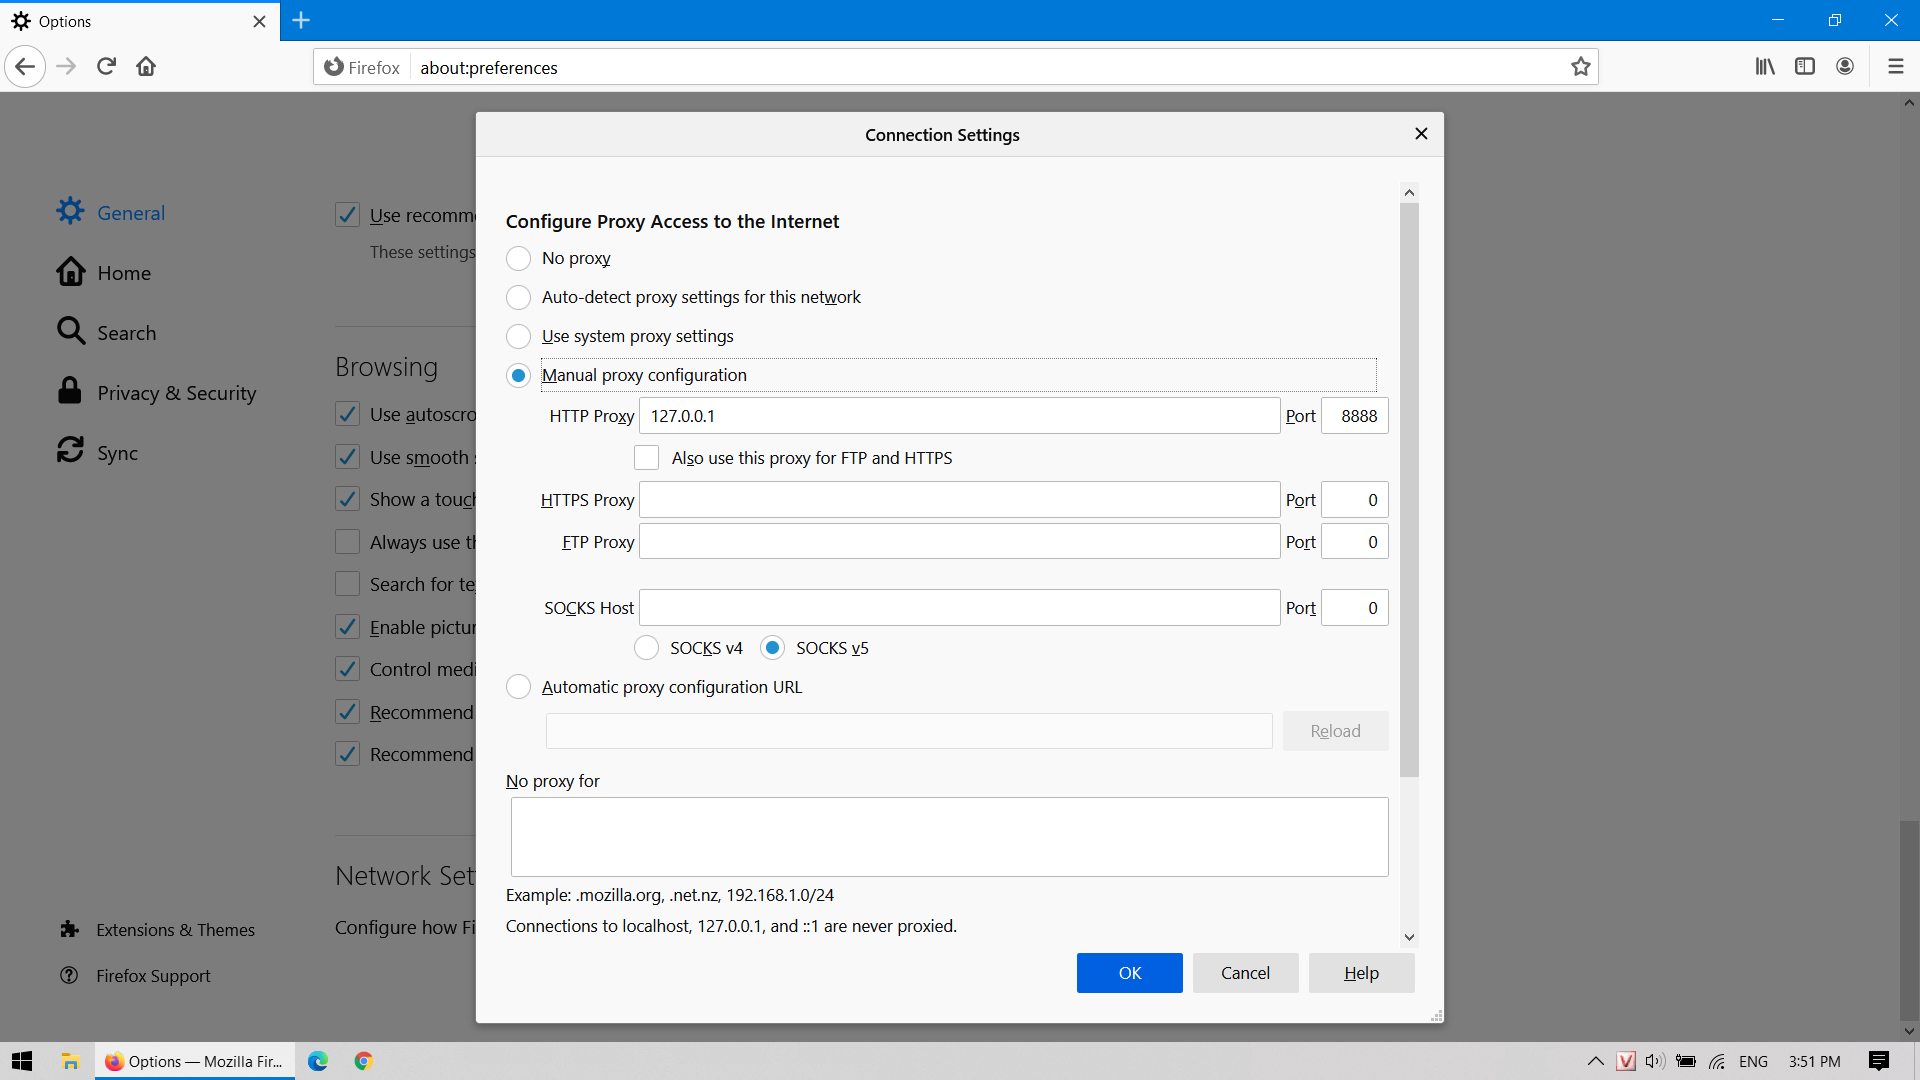
\includegraphics[scale=.25]{images/run_setting}
					\end{center}
					\caption{Cấu hình proxy server cho trình duyệt Mozilla Firefox}
				\end{figure}
			\end{center}
			\begin{itemize}
				\item Chọn Manual proxy configuration.
				\item Trong mục HTTP proxy nhập 127.0.0.1 là địa chỉ loop back.
				\item Trong mục Port tương ứng, nhập 8888 là port mà proxy server sẽ lắng nghe kết nối từ trình duyệt.
			\end{itemize}
		\subsection{File blacklist.conf}
			\begin{center}
				\begin{figure}[H]
					\begin{center}
						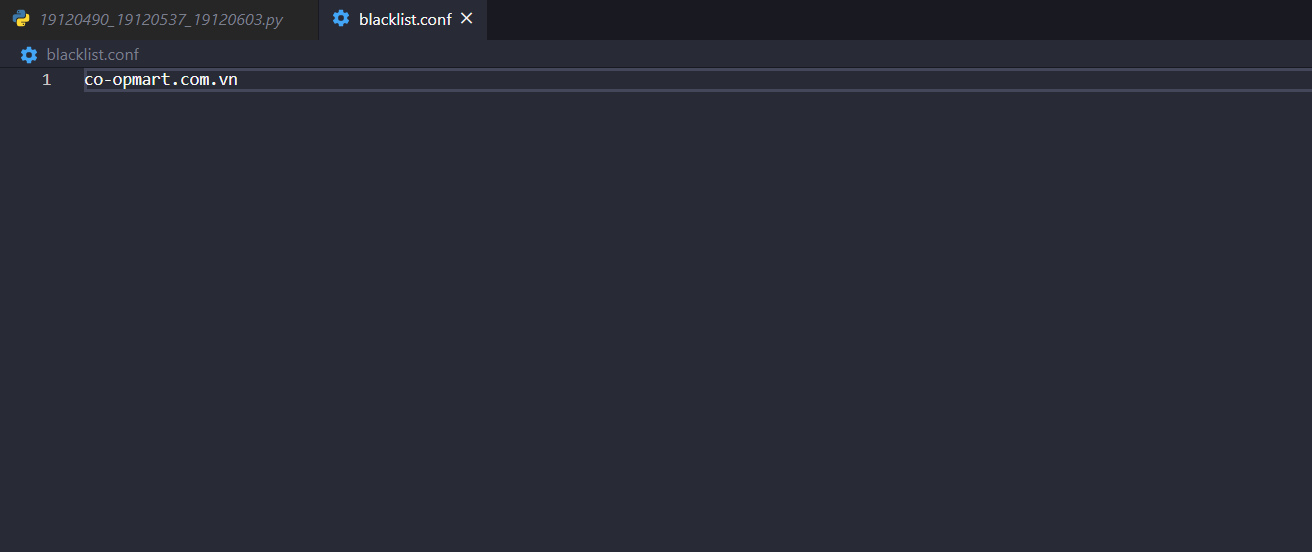
\includegraphics[scale=.49]{images/run_blacklist}
					\end{center}
					\caption{Nội dung file blacklist.conf}
				\end{figure}
			\end{center}
			\begin{itemize}
				\item Tạo một file blacklist.conf nằm cùng thư mục với file mã nguồn.
				\item Thêm vào đó co-opmart.com.vn là địa chỉ cần cấm.
			\end{itemize}
		\subsection{Chạy chương trình}
			\begin{itemize}
				\item Nếu dùng Visual Studio Code, cần cấu hình file .json cho Python để chạy trên console screen. Ngoài ra có thể dùng IDLE, Pycharm hay bất kỳ IDE, text editor nào khác.
				\item Tiến hành chạy (F5), ta được các thông số kết quả như khi đã cấu hình.
			\end{itemize}
			\begin{center}
				\begin{figure}[H]
					\begin{center}
						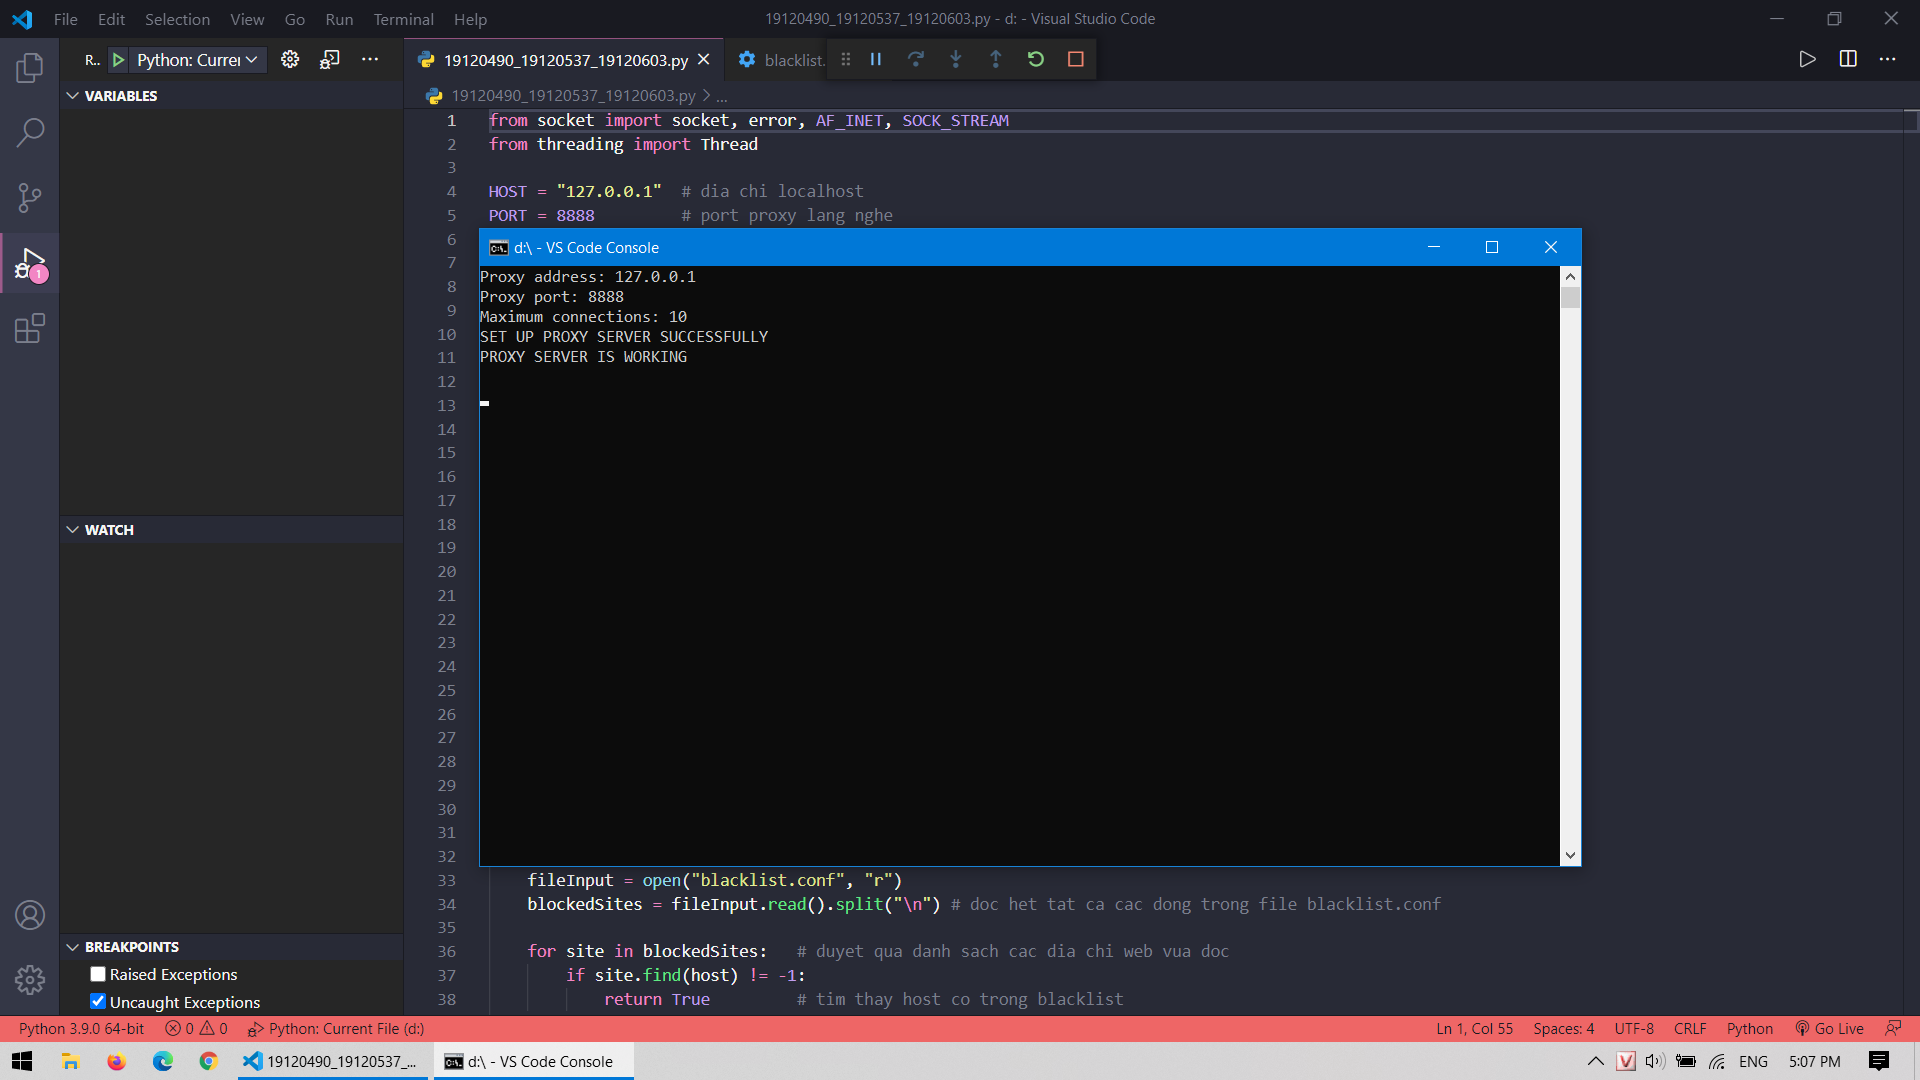
\includegraphics[scale=.25]{images/run_waiting}
					\end{center}
					\caption{Proxy server được thiết lập thành công, đang đợi kết nối}
				\end{figure}
			\end{center}
		\subsection{Truy cập một trang web (http)}
			Mở firefox, nhập vào thanh địa chỉ upcoder.hcmue.edu.vn, trong console screen hiện lên thông tin nhận trang web như hình dưới.
			\begin{center}
				\begin{figure}[H]
					\begin{center}
						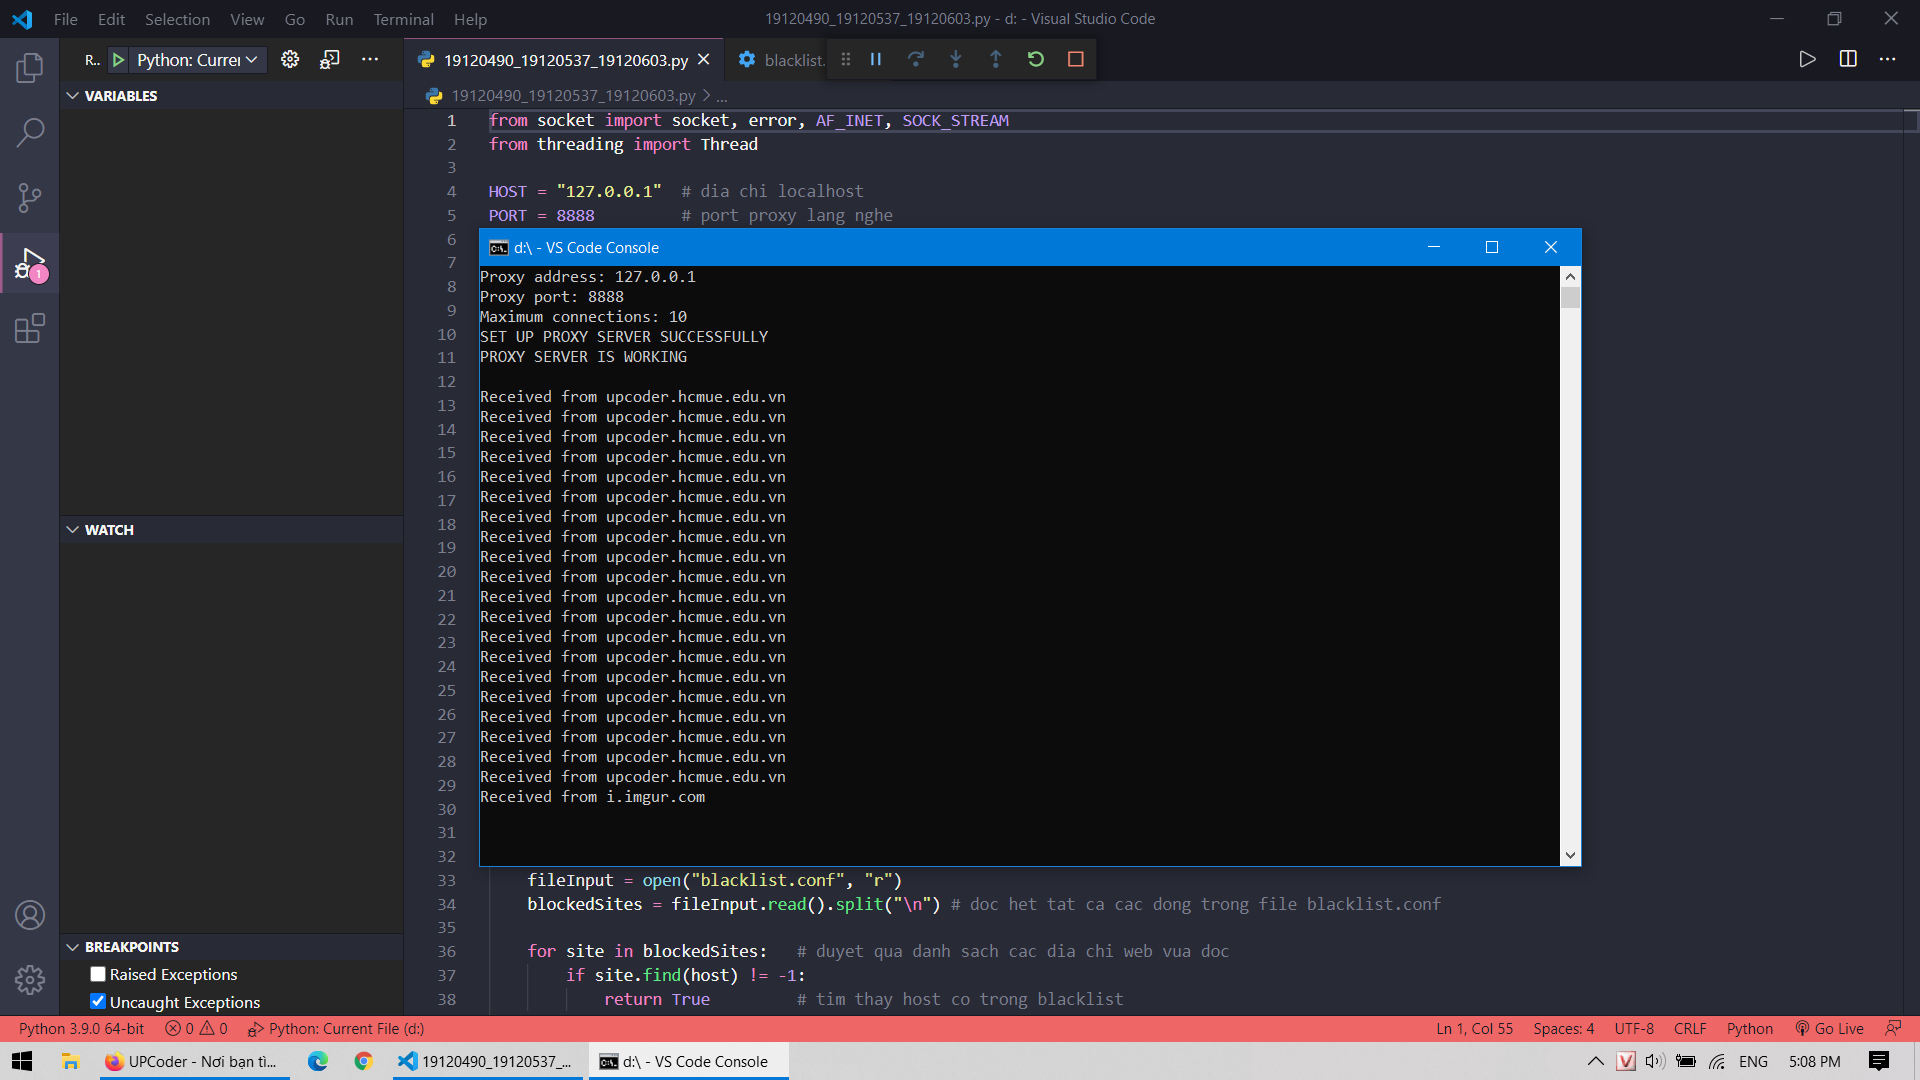
\includegraphics[scale=.25]{images/run_receiving}
					\end{center}
					\caption{Quá trình nhận các phần từ trang web upcoder.hcmue.edu.vn}
				\end{figure}
			\end{center}
			Kết quả proxy trả về cuối cùng là một trang web hoàn chỉnh được hiển thị lên trình duyệt.
			\begin{center}
				\begin{figure}[H]
					\begin{center}
						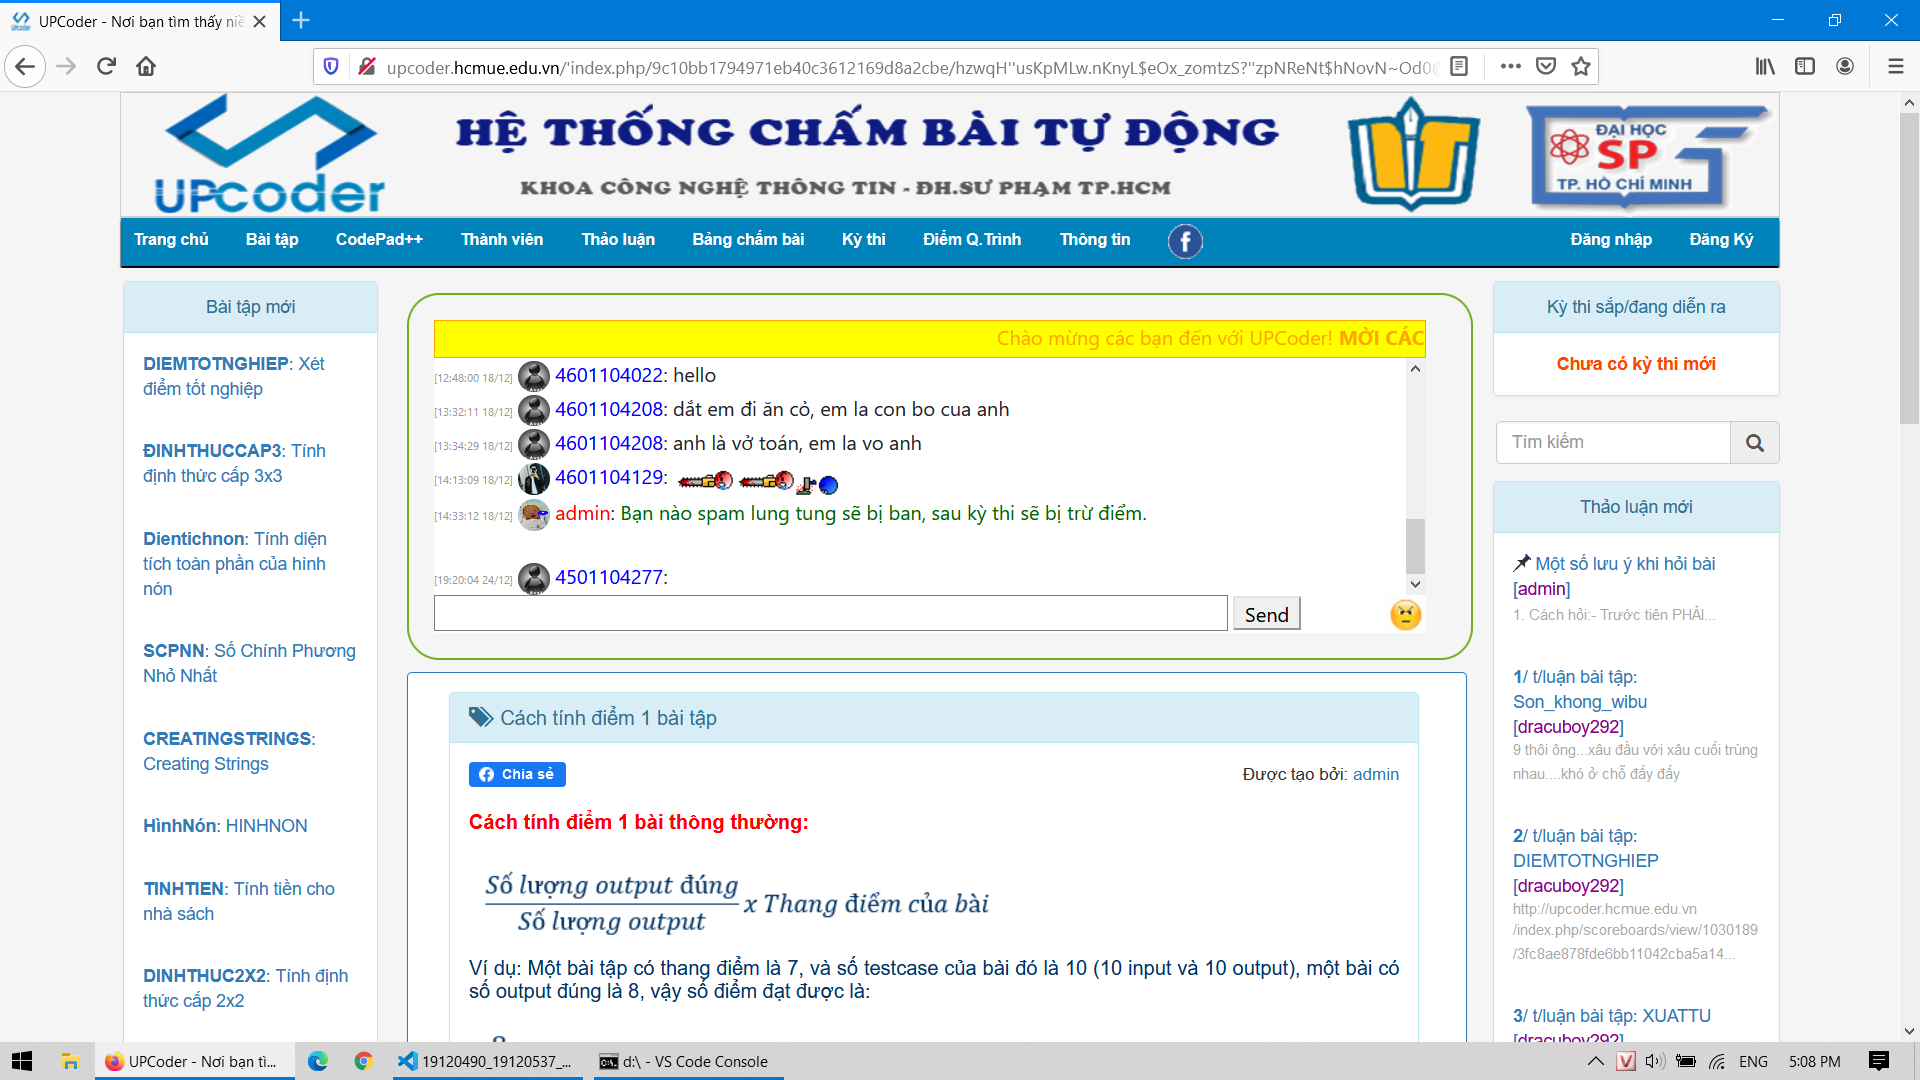
\includegraphics[scale=.25]{images/run_result}
					\end{center}
					\caption{Trang web kết quả từ request upcoder.hcmue.edu.vn}
				\end{figure}
			\end{center}
		\subsection{Cố tình truy cập một trang bị cấm}
			Tiếp tục, ta thử truy cập vào co-opmart.com.vn.
			\begin{center}
				\begin{figure}[H]
					\begin{center}
						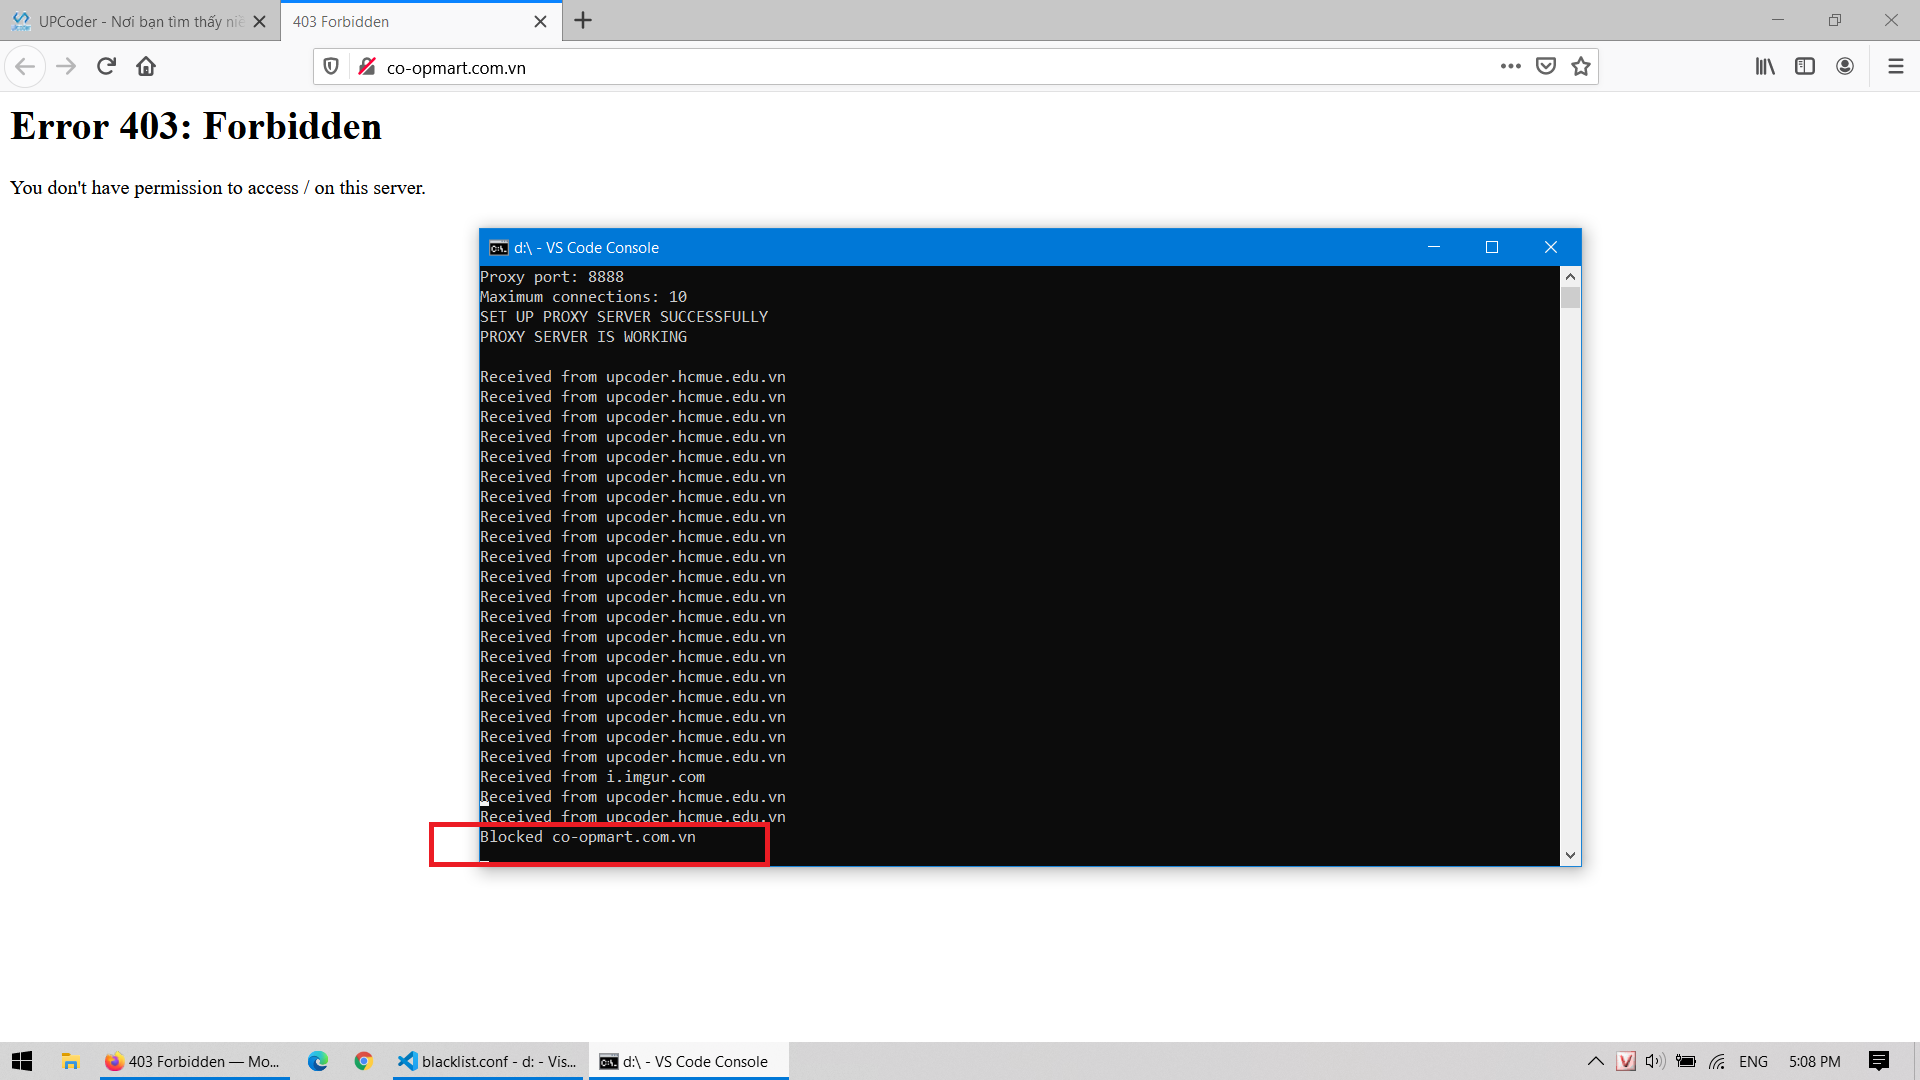
\includegraphics[scale=.335]{images/run_blocked}
					\end{center}
				\end{figure}
			\end{center}
			Vì trang này nằm trong blacklist.conf, nên khi truy cập, trong console screen chỉ nhận được thông báo rằng đã bị chặn. Phía trình duyệt, một trang HTML báo status Error 403: Forbidden được hiển thị.
	\section{Mức độ hoàn thành}
		\subsection{Chức năng làm được}
			\begin{itemize}
				\item Cho phép client truy cập website thông qua các phương thức GET, POST.
				\item Hỗ trợ cho giao thức HTTP.
				\item Xử lý đống thời các request từ client.
				\item Proxy server lắng nghe tại cổng 8888, chờ kết nối từ client.
				\item Chặn tất cả các truy cập đến các domain website có trong file blacklist.conf
			\end{itemize}
		\subsection{Chức năng chưa làm được}
			\begin{itemize}
				\item Không có.
			\end{itemize}
		\subsection{Mức độ hoàn thành}
			\begin{itemize}
				\item Hoàn thành 100\% các yêu cầu của đồ án.
			\end{itemize}
	\section{Bắt gói tin bằng Wireshark}
		\begin{center}
			\begin{figure}[H]
				\begin{center}
					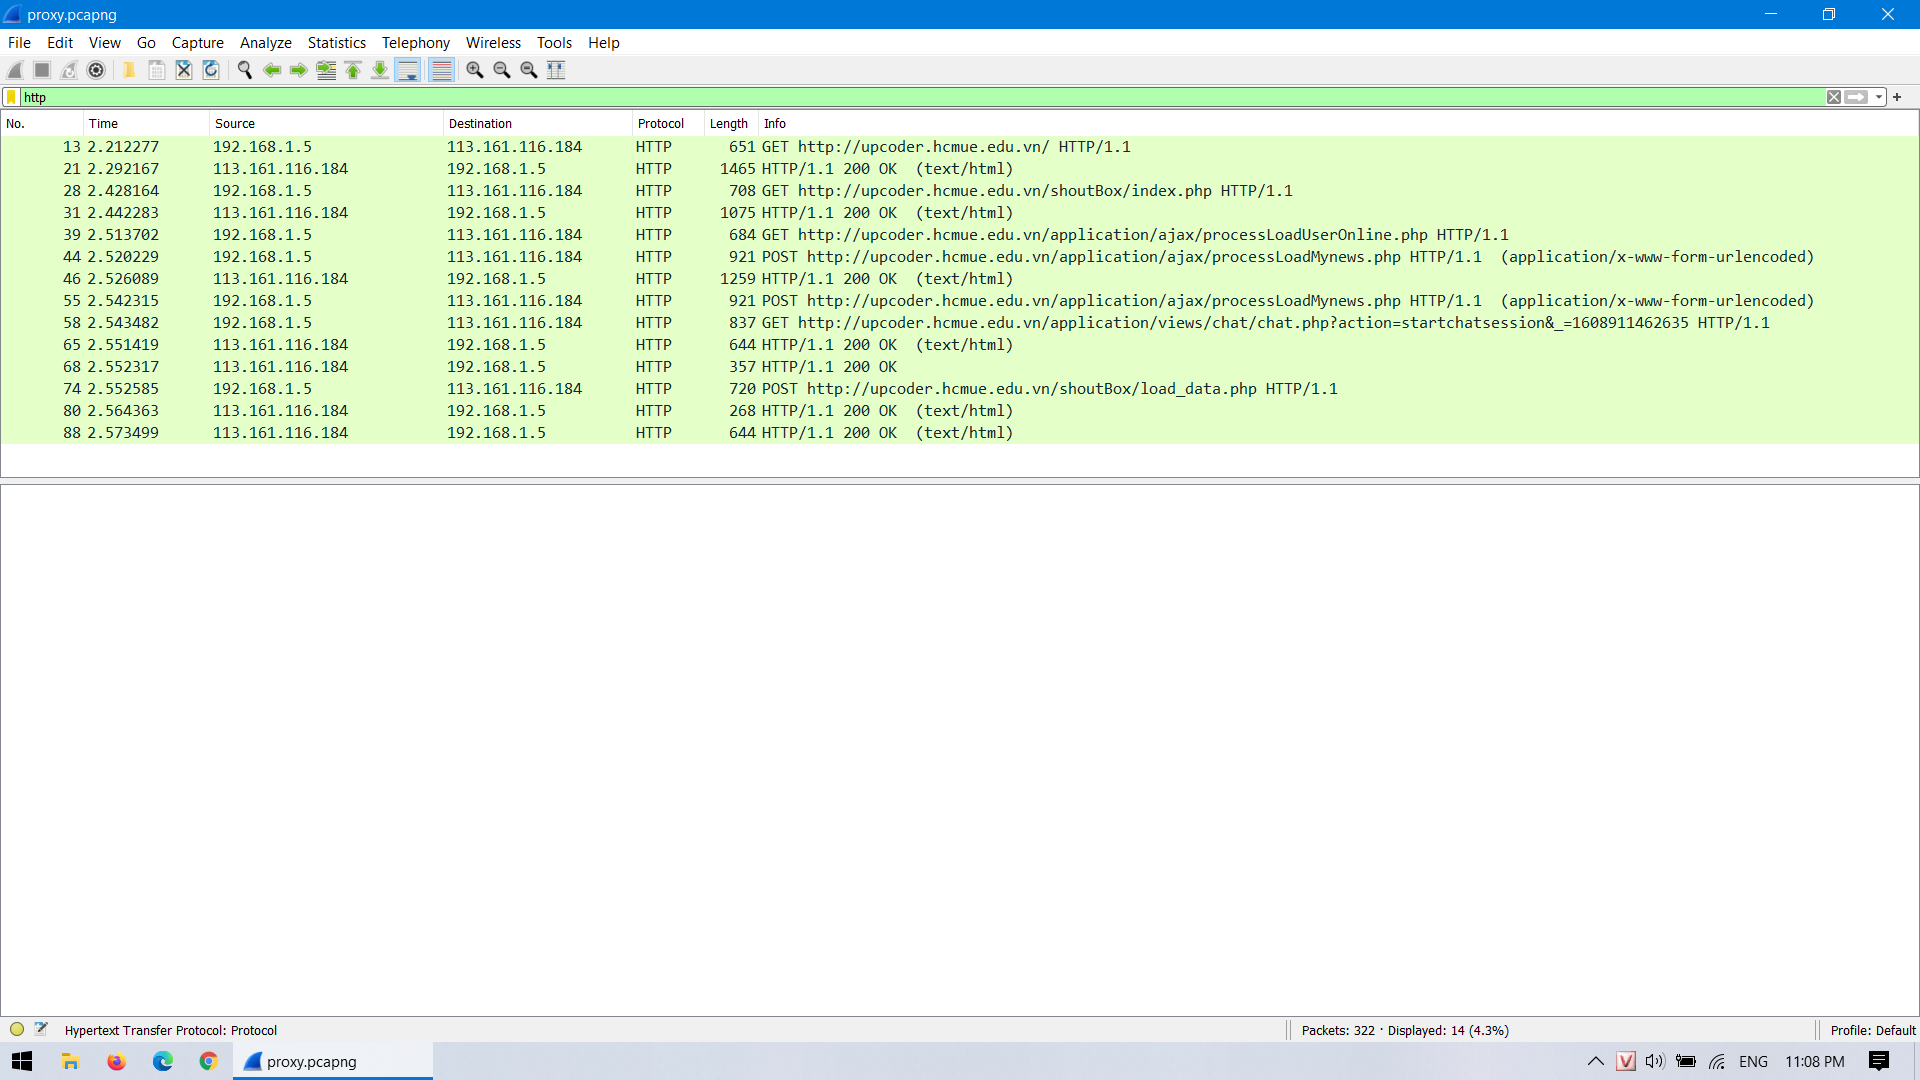
\includegraphics[scale=.25]{images/ws_packets}
				\end{center}
				\caption{Các gói tin HTTP bắt được khi truy cập upcoder.hcmue.edu.vn}
			\end{figure}
		\end{center}
		\begin{center}
			\begin{figure}[H]
				\begin{center}
					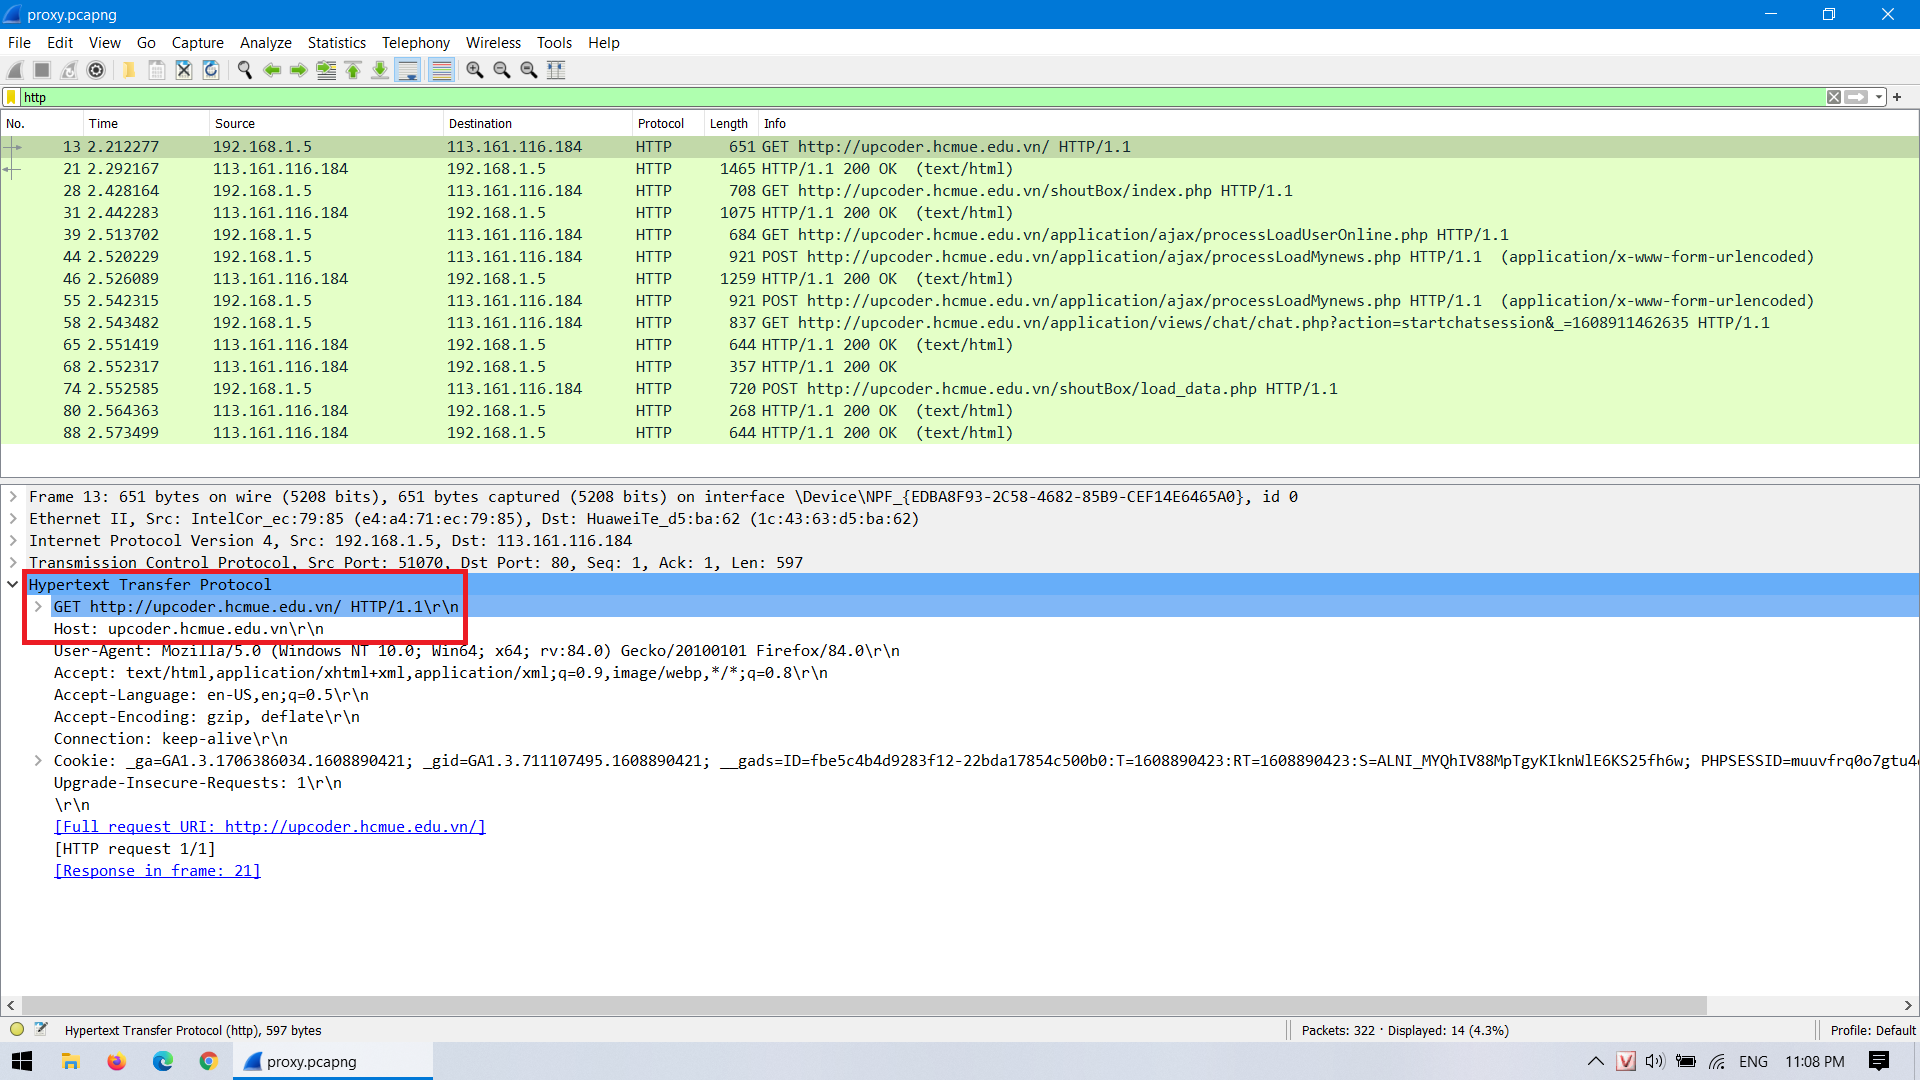
\includegraphics[scale=.335]{images/ws_request}
				\end{center}
				\caption{Cấu trúc một gói tin HTTP request}						
			\end{figure}
		\end{center}
		\begin{center}
			\begin{figure}[H]
				\begin{center}
					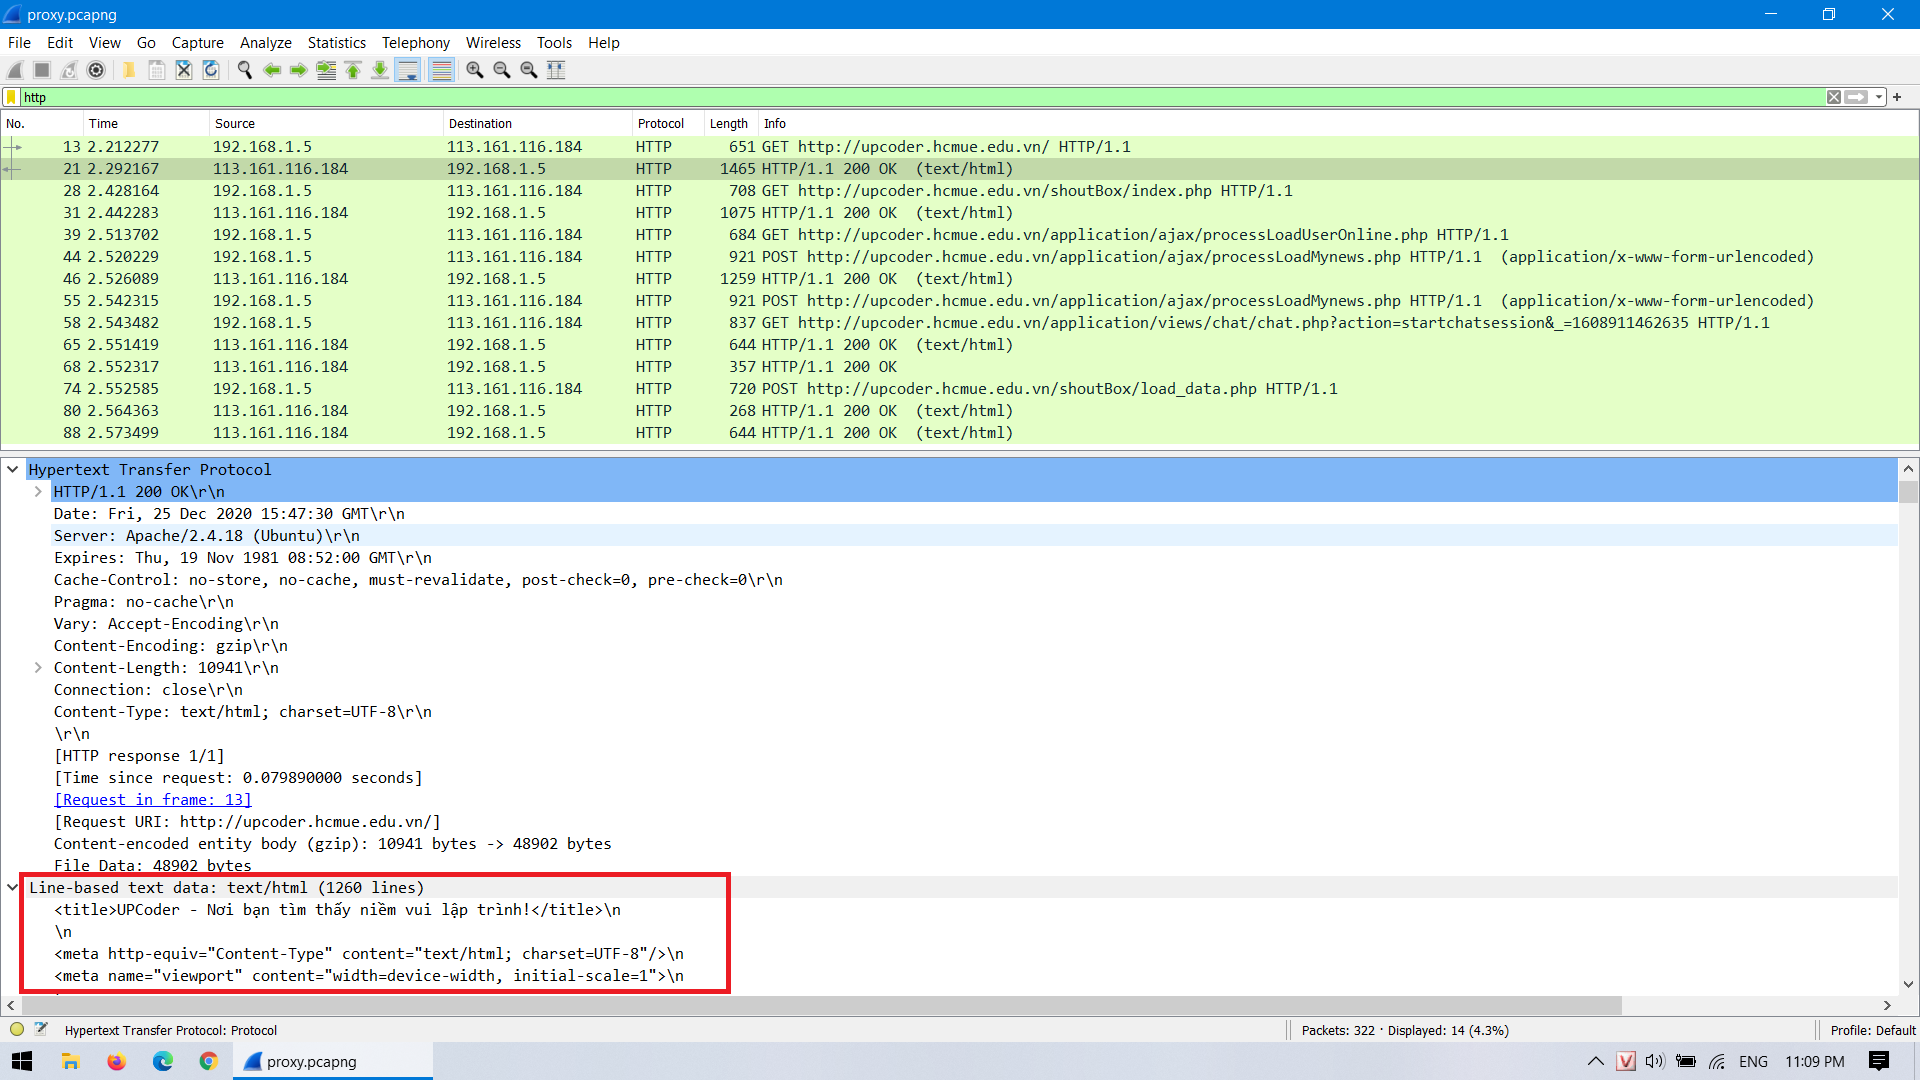
\includegraphics[scale=.335]{images/ws_response}
				\end{center}
				\caption{Cấu trúc một gói tin HTTP response và phần trang web trả về}
			\end{figure}
		\end{center}
		Quá trình nhận dữ liệu giữa client - proxy server và proxy server – web server:
		\vskip.1in
		\begin{itemize}
			\item Khi bắt đầu thao tác truy cập website, client sẽ gửi một request đến proxy server.
			\item Proxy server lấy ra những thông tin bao gồm host, port (\textit{Hình 7}) từ gói HTTP request nhận từ client, sau đó kiểm tra host có nằm trong danh sách bị cấm hay không. Nếu có thì gửi gói HTTP 403 Forbidden về cho client, quá trình duyệt trang web dừng tại đây. Nếu không thì proxy server chuyển tiếp gói HTTP request lên web server.
			\item Sau đó web server sẽ gửi gói HTTP response cho proxy server (\textit{Hình 8}).
			\item Proxy server chuyển tiếp gói HTTP response này đến cho client.
			\item Cứ như vậy, client gửi lần lượt từng gói HTTP request và nhận về từng gói HTTP response cho đến khi được một trang web hoàn chỉnh.
		\end{itemize}
	\section{Proxy Server trong thực tế}
		\subsection{Lọc nội dung truy cập (content filtering)}
			Ứng dụng này của proxy server đã được minh họa một cách đơn giản trong đồ án, bằng việc cấu hình một file blacklist.conf và cấm bất cứ request nào gửi về các host có trong file, proxy server đã lọc được các trang mà các máy trong mạng cục bộ không được phép truy cập. Trong thực tế cơ chế hoạt động cũng tương tự nhưng hệ thống phức tạp hơn.
		\subsection{Giám sát truy cập (monitoring)}
			Ngoài việc lọc bỏ các request, proxy server có thể giám sát truy cập của các máy trong mạng cục bộ, vì các request và response đều đi qua proxy. Do đó có thể dễ dàng kiểm tra được nội dung truy cập của các client.
		\subsection{Bảo mật thông tin (privacy)}
			\begin{itemize}
				\item Người dùng trong mạng cục bộ có thể kết nối với trang web bên ngoài thông qua proxy server thay vì kết nối trực tiếp. Như vậy, bất kỳ request nào đi qua proxy server chỉ được web server hiểu là đến từ proxy đó, web server không biết thông tin, IP của các máy nằm đằng sau proxy server. Điều này cho phép các máy trong mạng cục bộ kết nối ẩn danh với Internet, giúp tăng cường bảo mật cho hệ thống.
				\item Do trong đồ án này proxy server chạy trực tiếp trên client, nên ứng dụng này không được thể hiện.
			\end{itemize}
		\subsection{Giảm thời gian tải trang, tiết kiệm băng thông (caching)}
			\begin{itemize}
				\item Trong thực tế, proxy server luôn hỗ trợ chức năng caching. Nó tải bản sao của một trang web thường truy cập xuống và lưu vào bộ nhớ đệm (cache). Các bản sao luôn được kiểm tra và cập nhật mới nhất như trên web server.
				\item Các trang web caching này có thể được truy cập bất cứ lúc nào, bởi bất kỳ các máy nào sử dụng chung proxy server, mà không cần trực tuyến. Như vậy, caching làm giảm độ trễ khi tải trang cũng như tiết kiệm băng thông.
			\end{itemize}
	\section{Tham khảo}
		\begin{itemize}
			\item https://www.youtube.com/watch?v=Lhxwh30kqQ0\&t=159s\&ab\_channel=Devsec
			\item https://luugiathuy.com/2011/03/simple-web-proxy-python/
			\item https://realpython.com/intro-to-python-threading/
			\item https://wheelhouse.solutions/the-benefits-of-using-a-network-proxy-server/
			\item https://www.rswebsols.com/tutorials/technology/proxy-server-advantages-disadvantages
		\end{itemize}
\end{document}